\documentclass{article}
\usepackage[utf8]{inputenc}
\usepackage{graphicx}
\usepackage{wrapfig}
\usepackage{caption}


\begin{document}

\section{Connexion à Office 365 et Teams}

Nikolai

Possibilité de télécharger l'application

\section{Apparence de la page d'accueil}

La page d'accueil de Teams se présente sous forme d'une liste de classes 

\begin{figure}[h]
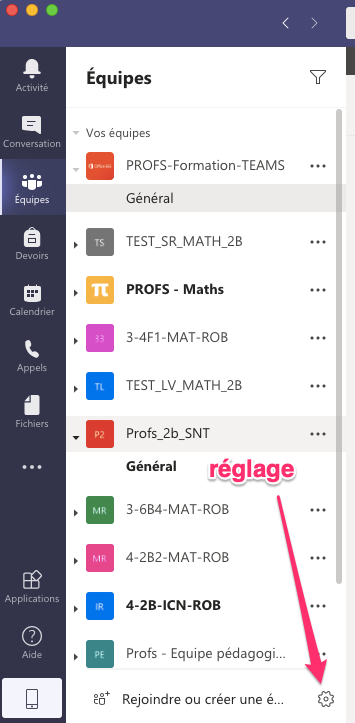
\includegraphics[width=5cm]{accueil_liste.png}
\centering
\end{figure}

ou sous forme d'une grille de classes \newpage

\begin{figure}[h]
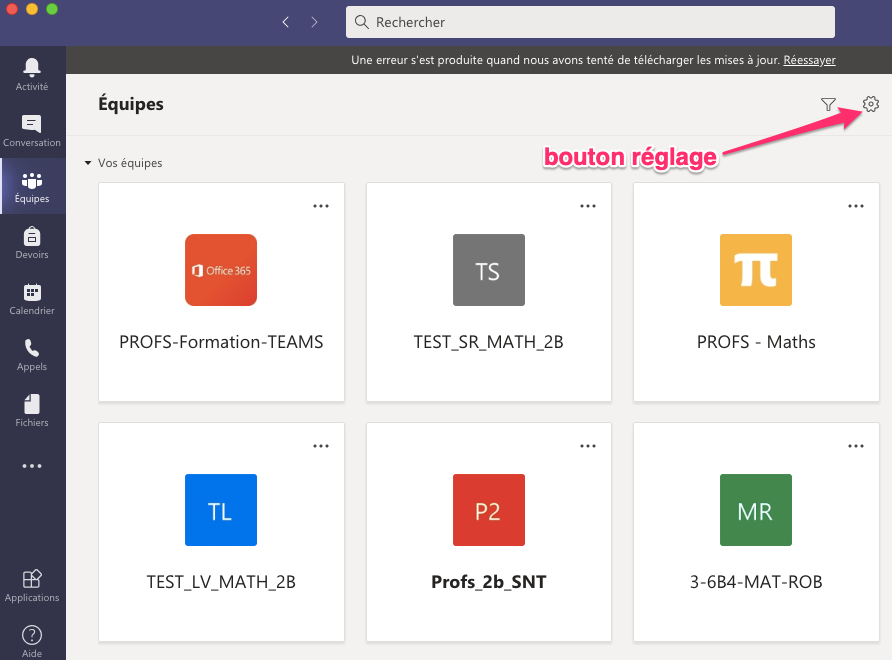
\includegraphics[width=10cm]{accueil_grille.png}
\centering
\end{figure}

Pour passer d'une forme à l'autre, il faut cliquer sur le sigle 
\includegraphics[width=0.7cm]{bouton_parametres.png}, choisir \textit{Changer d'affichage} dans le menu déroulant, comme dans l'exemple illustré ci-dessous :

\begin{figure}[h]
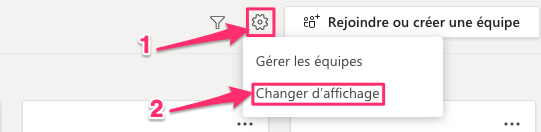
\includegraphics[width=10cm]{changement_liste.png}
\centering
\end{figure}

il faut ensuite sélectionner le type d'affichage souhaité entre \textit{Grille} et \textit{Liste}
\newpage

\begin{figure}[h]
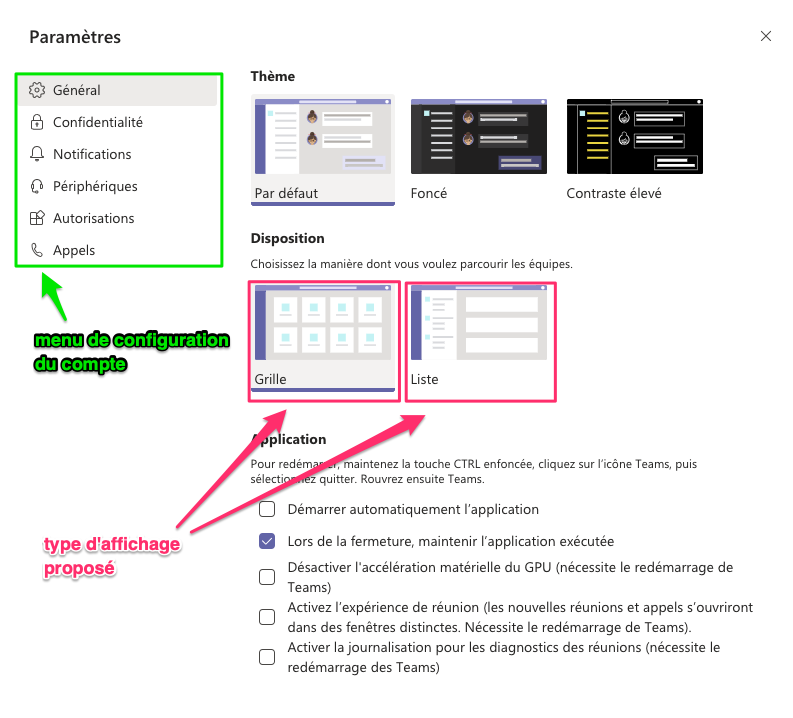
\includegraphics[width=12cm]{choix_parametre.png}
\centering
\end{figure}

 Pour entrer maintenant dans votre classe, dans la matière de votre choix, il suffit de cliquer sur l'icône correspondante

\begin{figure}[h]
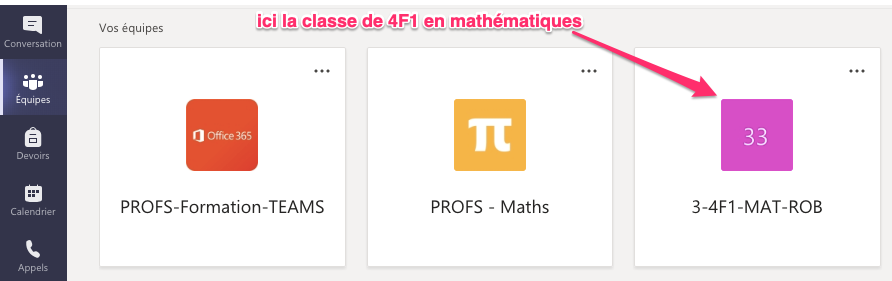
\includegraphics[width=12cm]{entree_classe.png}
\centering
\end{figure}

\newpage

\section{Utilisation de la messagerie}

La messagerie instantanée proposée par Teams doit permettre aux élèves et aux enseignants de communiquer en dehors de l'école dans un cadre qui reste strictement scolaire. Ainsi les messages personnels n'ont aucune raison d'être sur Teams. Il n'est par ailleurs pas possible pour un élève de supprimer un message envoyé. Seul le modérateur de la classe peut procéder à une telle suppression. 

Par ailleurs, toute forme d'insulte, de jugement personnel ou de critique envers un membre de la classe est à proscrire.



\section{Consulter et télécharger un document}

Nikolai

\section{Déposer un devoir}

Pour consulter les devoirs déposés par votre enseignant, il faut choisir \textit{2 de plus} dans la barre de menus du haut de page, puis sélectionner \textit{Devoirs}.

\begin{figure}[h]
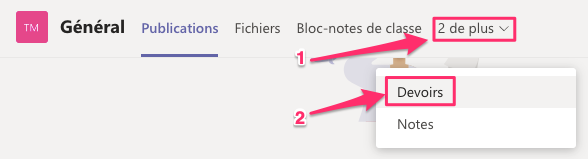
\includegraphics[width=10cm]{devoir1.png}
\centering
\end{figure}

La page qui s'affiche maintenant fait le bilan de ce qui a déjà été fait et des devoirs proposés par votre enseignant. En cliquant sur \textit{Rédaction} vous pourrez accéder au devoir.

\begin{figure}[h]
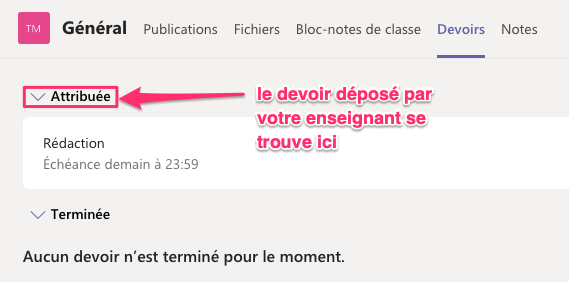
\includegraphics[width=10cm]{devoir2.png}
\centering
\end{figure}

\newpage
 Vous obtenez alors l'écran suivant

\begin{figure}[h]
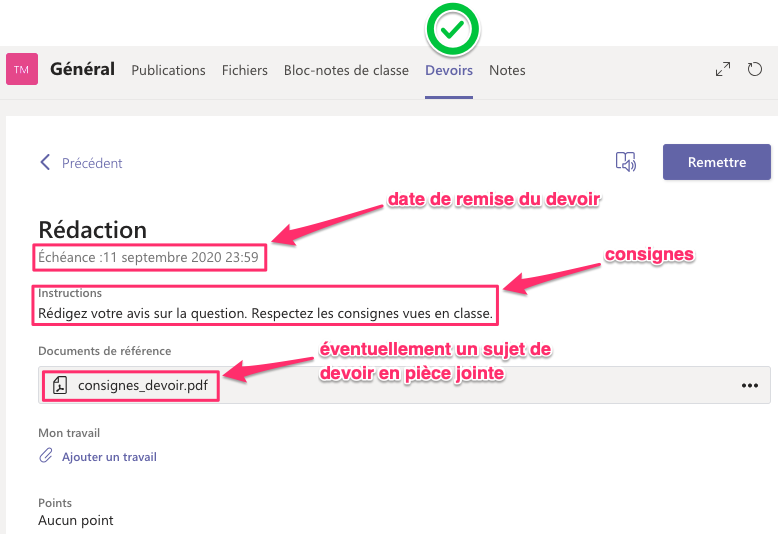
\includegraphics[width=12cm]{devoir3.png}
\centering
\end{figure}

Il est maintenant possible de consulter le sujet sous forme de pièce jointe en sélectionnant ...

\section{Accéder à mon carnet}

\section{Rejoindre une visio-conférence}


\end{document}